\chapter{Efficient Encoding, Decoding, and Indexing} \label{chap:coding}
The mappings described in the previous chapter are only one part of the process for associating geospatial data to cells of a 3D DGGS.
With geospatial data mapped to the domain of the grid system, the set of cells associated with the geometry of the data---and the indices of said cells---must be obtained.
As described earlier, this entire process is known as grid encoding.
Likewise, there needs to be a process to obtain the geometry of a cell (in grid space) from its index, so that the geometry can be mapped to the corresponding cell geometry in physical space.
This process is known as grid decoding.


Beyond encoding and decoding, there are also operations and queries done with a DGGS directly in grid space.
These operations often use algorithms for traversing the grid through neighbour, parent, and child relationships between cells.
Thus, queries that give these relationships for a given cell are another essential component of a fully functioning DGGS.


This chapter completes the 3D DGGS's described in the preceding chapters by providing encoding, decoding, and indexing operations for the SDOG modifications and grid extension method.
Different types of geometry typically require their own encoding algorithms.
In this thesis, we focus on point encoding as it is the most fundamental, with the encoding of more complex geometries built off this operation.
While SDOG already has hierarchical coding algorithms~\cite{yu2009sdog, yu2009coding} that are trivially adapted to work with the modified grids, we derive constant time alternatives that work for both the conventional grid and our modifications.
For completeness, we also describe algorithms for performing neighbour, parent, and child queries.
For the grid extension method, we derive these operations in such a way as to ensure interoperability and consistency between the 3D and input DGGS.


\section{SDOG}
When first introduced by Yu and Wu, the authors proposed two indexing schemes for use with SDOG~\cite{yu2009coding}.
These schemes are both based on a modified Morton code (also known as a Z-order curve)~\cite{morton1966computer}; however, one is intended for indexing a single resolution whereas the other for the full cell hierarchy.
We focus on the hierarchical scheme, as grid \textit{systems} are the main focus of this thesis.


\begin{figure}[ht!]
	\centering
	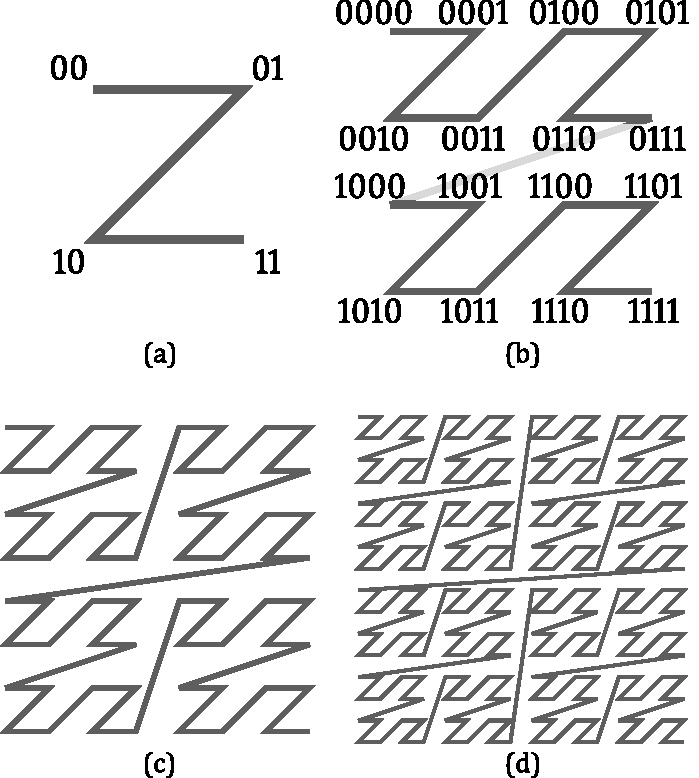
\includegraphics[width=0.6\textwidth]{morton-multiple.pdf}
	\caption[Four resolutions of Morton codes]{
		The first four resolutions of Morton codes for a quadtree.
		(a)--(d) show resolutions 1--4, respectively.
		Modified from~~\cite{morton-multiple}; original image courtesy of David Eppstein -- CC BY-SA 3.0
	}
	\label{fig:morton-multiple}
\end{figure}


Figure~\ref{fig:morton-multiple} demonstrates Morton coding for four resolutions of a conventional Euclidean quadtree.
Indices are assigned consecutively, starting at zero, to cells in the order the curve passes through them.
The resulting indices are hierarchical, where the index of a cell is that of its parent with its local index---obtained relative to its parent---appended.
While shown for a quadtree (2D), Morton codes generalize to any integer dimension $n$.
In this case, each cell has $2^n$ children, which means $n$ bits are needed to represent each uniquely.
Thus, from a given cell index, the resolution of the grid that cell appears at is the bit width of the index divided by $n$.
For a fixed-width representation of indices, a leaded bit set to one marks the start of the actual index.


\begin{figure}[htp!]
	\centering
	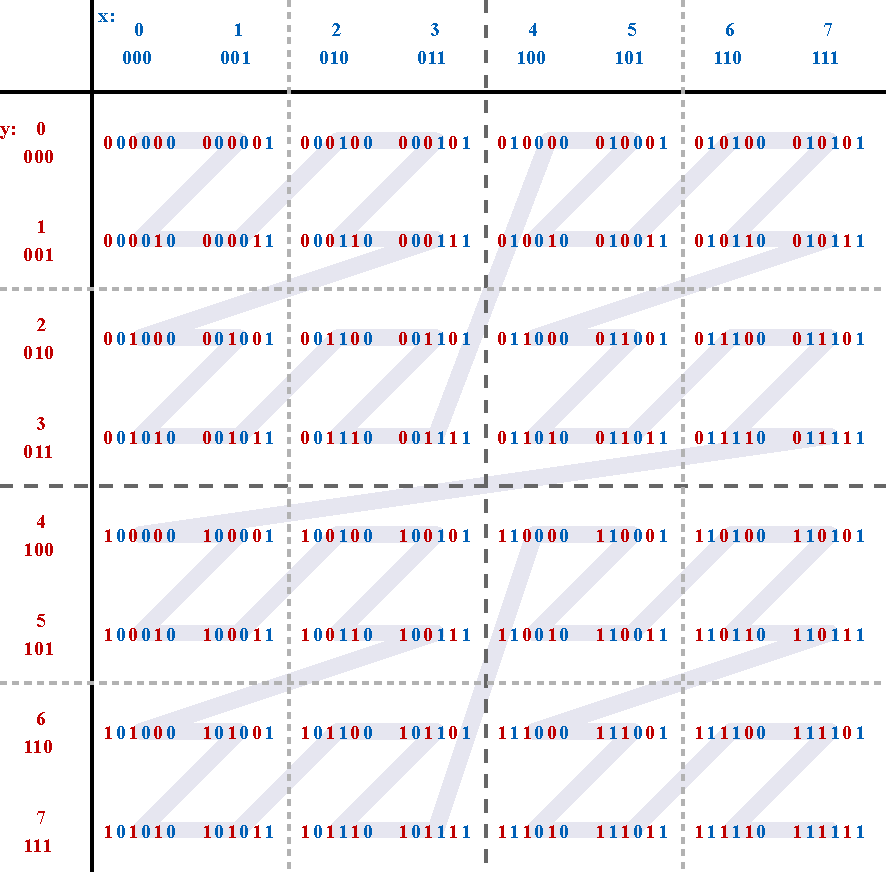
\includegraphics[width=\textwidth]{morton-interleave.pdf}
	\caption[Morton codes by bit-interleaving]{
		Third resolution Morton codes and their respective coordinate indices.
		Note how the Morton codes are obtained by interleaving the bits of the coordinate indices.
		In this figure, the $x$ coordinate is traversed first by the curve, so it is the lowest order bit in the Morton code.
		Image courtesy of David Eppstein~\cite{morton-interleave} -- CC BY-SA 3.0
	}
	\label{fig:morton-interleave}
\end{figure}


One benefit of Morton codes over more local space-filling curves---such as the Hilbert curve---is the ease at which a multi-dimensional index is encoded and vice versa.
As demonstrated in Figure~\ref{fig:morton-interleave}, the Morton code is obtained simply by interleaving the bits of the coordinate indices; likewise, unweaving the bits of a Morton code gives the coordinate indices.
While these are not constant-time operation in general, magic numbers and lookup tables allow them to be done efficiently and in constant time for a fixed bit width~\cite{bit twiddle, libmorton}.


\begin{figure}[ht!]
	\centering
	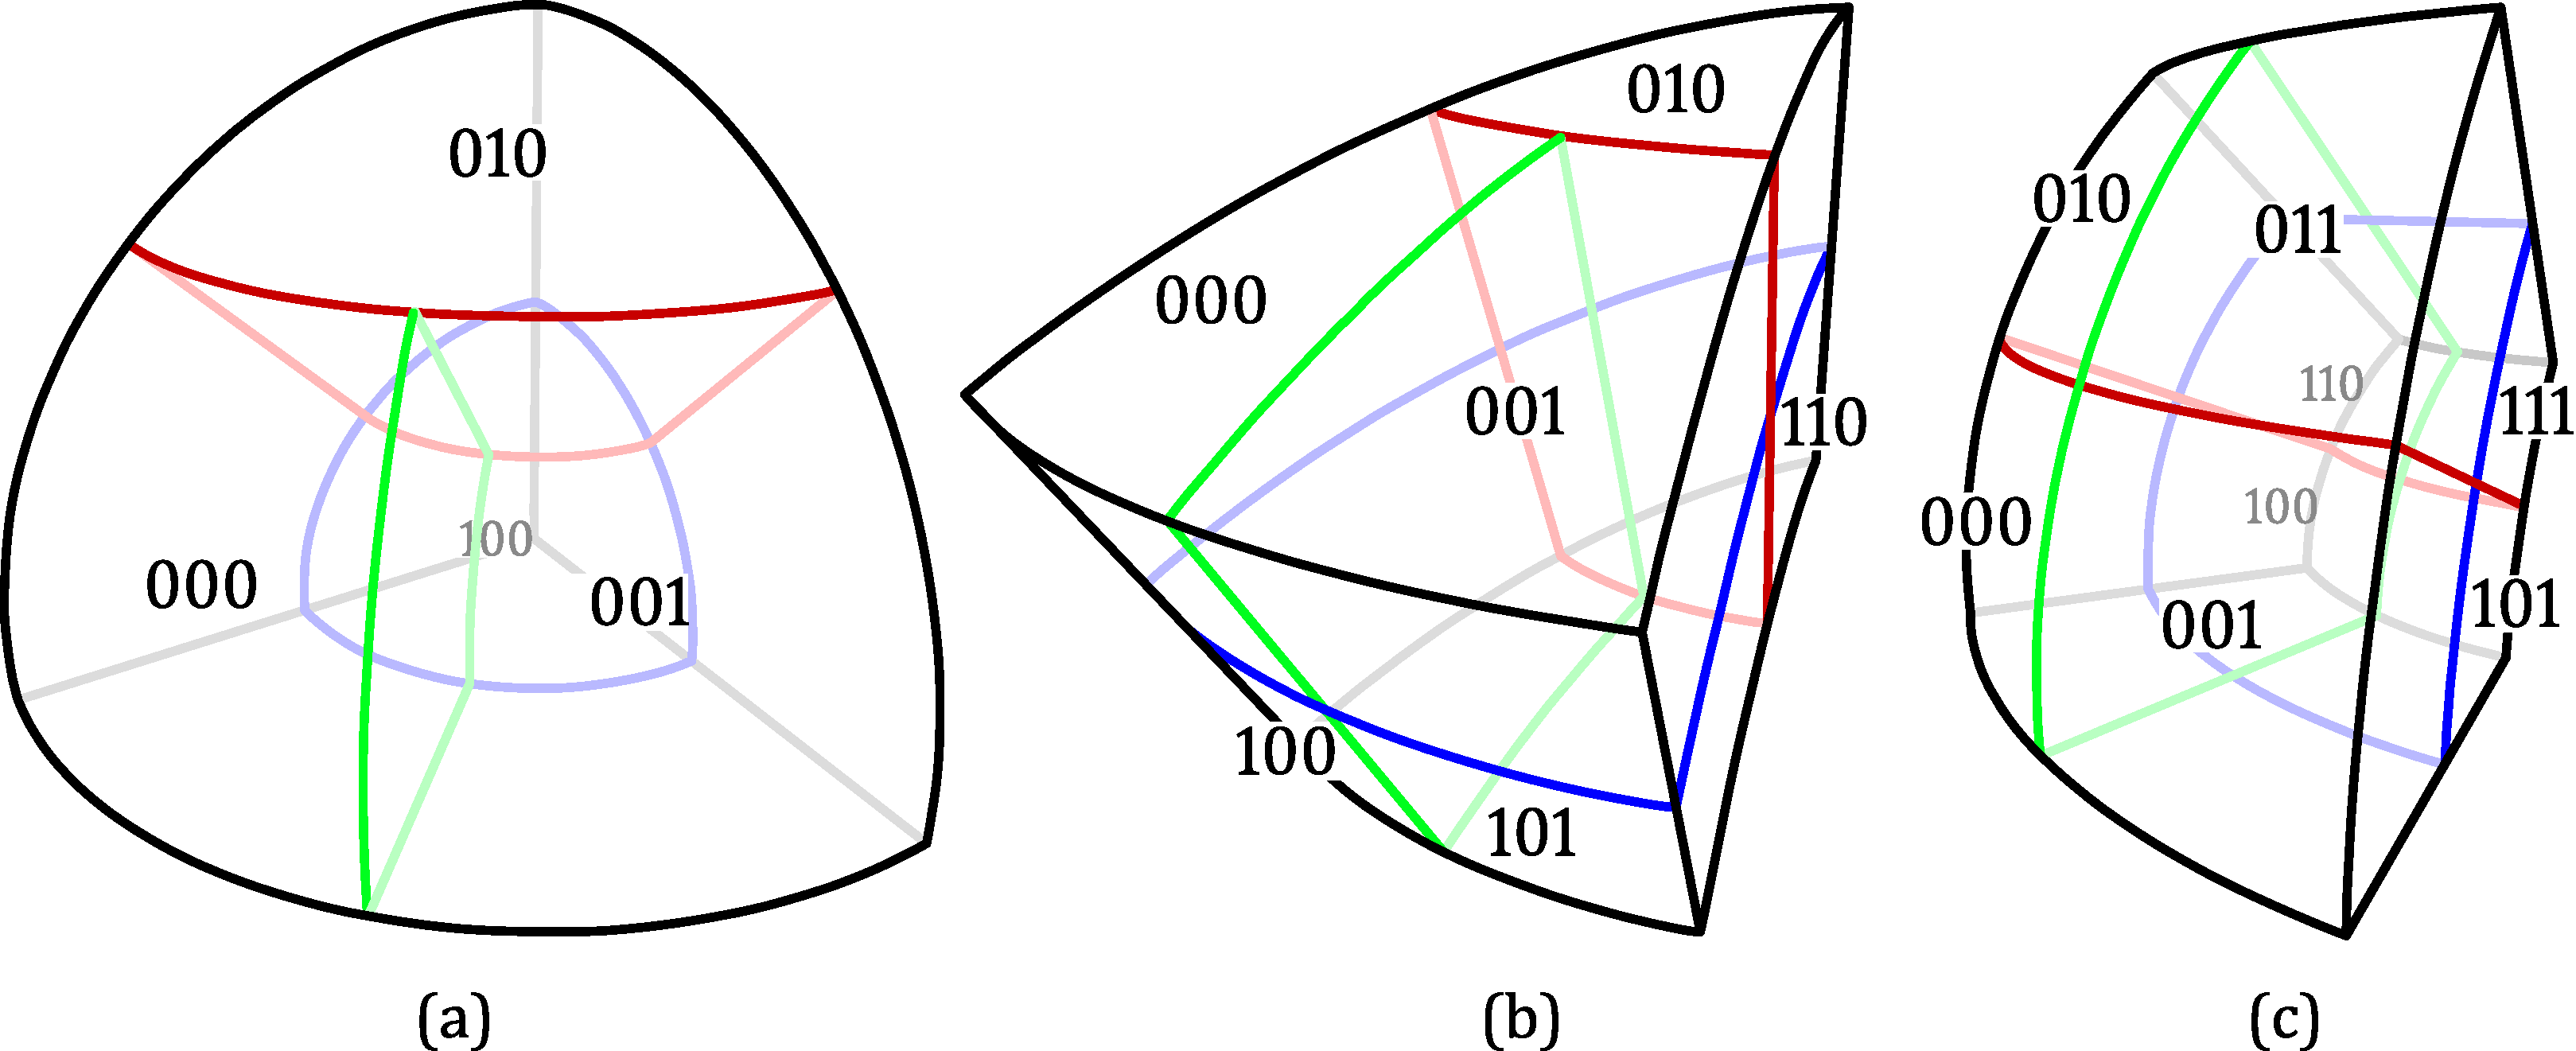
\includegraphics[width=\textwidth]{sdog-dmc.pdf}
	\caption[Degenerate Morton codes for the different SDOG cell types]{
		Degenerate Morton codes for (a) SG cells, (b) LG cells, and (c) NG cells.
	}
	\label{fig:sdog-dmc}
\end{figure}


Due to the semiregular degenerate nature of SDOG, Morton coding must be modified for use with the grid system.
First, Morton coding for a cell's children is done as if refinement is entirely regular.
For NG cells, refinement \textit{is} regular, and no modifications are needed.
However, for SG and LG cells, some of these codes will refer to the same cell.
In these cases, we merge duplicate codes with the lower value kept.
We call this the degenerate Morton code (DMC).
Figure~\ref{fig:sdog-dmc} shows the child codes of cells for each SDOG cell type.
In this scheme, the different spherical coordinates are traversed in the order (1) longitude---small to large (2) latitude---small to large (3) radius---large to small.
Finally, to distinguish between the eight octants, each is given a unique identifier: the octant code.
The full index of an SDOG cell consists of the octant code and DMC, concatenated, along with a leading one for fixed-width representations.
For the remainder of this chapter, we assume the use of a fixed-width integer for representing SDOG indices.


From the above definition, we know the number of bits needed to represent an SDOG index at refinement level $k$ is $3k + 4$.
Likewise, given an index with width $\omega$, the refinement level of that cell is $(\omega - 4) / 3$.
We use this property below to obtain $k$ for the decoding algorithms, implicitly.


\subsection{Hierarchical Algorithms}
We first give a brief overview of the hierarchical coding algorithms for SDOG, as these will be the baseline for evaluating our proposed ones.
Hierarchical coding works by traversing the grid system one resolution at a time, using the refinement rules for the relevant cell at each iteration.
As a result, these types of algorithms are linear on the level of refinement.
However, because they use refinement rules directly, they are trivially modified to work for our SDOG modifications by simply changing the refinement used in the algorithms accordingly.


\subsubsection{Encoding}
The algorithm for hierarchical point encoding with SDOG is given in Algorithm~\ref{alg:encode}.
The input is a point $p$ and resolution $k$; the output is the index $i$ of the cell that contains $p$ at $k$.


\begin{algorithm}
	\caption{Hierarchical point encoding for SDOG}
	
	\begin{algorithmic}
		
		\STATE determine which octant contains $p$
		\STATE cellBoundaries $\leftarrow$ boundaries of octant
		\STATE currCellType $\leftarrow$ SG
		\STATE $i \leftarrow \operatorname{append}(1, \mathrm{octantCode})$
		
		\FOR{$k$ iterations}
		\STATE use refinement rules for currCellType with cellBoundaries to find child cells
		\STATE determine which child contains $p$
		\STATE cellBoundaries $\leftarrow$ boundaries of child
		\STATE currCellType $\leftarrow$ type of child
		\STATE $i \leftarrow \operatorname{append}(i, \mathrm{child~index})$
		\ENDFOR
		\RETURN $i$
		
	\end{algorithmic}
	\label{alg:encode}
\end{algorithm}


\subsubsection{Decoding}
The algorithm for hierarchical decoding with SDOG is given in Algorithm~\ref{alg:decode}.
The input is an index $i$; the output is the cell boundaries of $i$.


\begin{algorithm}
	\caption{Hierarchical cell decoding for SDOG}
	
	\begin{algorithmic}
		
		\STATE determine octant from $i$
		\STATE cellBoundaries $\leftarrow$ boundaries of octant
		\STATE currCellType $\leftarrow$ SG
		\STATE remove highest four bits of $i$
		
		\FOR{$k$ iterations}
		\STATE use refinement rules for currCellType with cellBoundaries to find child cells
		\STATE $c \leftarrow$ highest three bits of $i$
		\STATE remove highest three bits of $i$
		\STATE determine which child cell matches $c$
		\STATE cellBoundaries $\leftarrow$ boundaries of $c$
		\STATE currCellType $\leftarrow$ type of $c$
		\ENDFOR
		\RETURN cellBoundaries
		
	\end{algorithmic}
	\label{alg:decode}
\end{algorithm}


\subsection{Direct Algorithms}
For a uniform grid, coordinate indices are trivially obtained in constant time.
Key pieces are to know the number of cells and range of values.
Semiregular regions of SDOG are uniform grids.
Thus, if we know which semiregular region is relevant for the operation being done, we can operate in constant time.
Coordinate indices are then used with bit interleaving and unweaving described earlier to get full DMC.


\subsubsection{Encoding}
Explanation goes here.

\begin{equation*}
\hat{r} = \frac{r}{R_\mathrm{max}}
\end{equation*}

\begin{equation*}
\hat{\varphi} = \frac{2 \varphi}{\pi}
\end{equation*}

\begin{equation*}
\hat{\lambda} = \frac{2 \lambda}{\pi}
\end{equation*}

\begin{equation*}
s = \lfloor \log_{0.5} \hat{r} \rfloor
\end{equation*}

\begin{equation*}
z = \lfloor \log_{0.5} ( 1 - \hat{\varphi} ) \rfloor
\end{equation*}

\begin{equation*}
k_\varphi = \min ( s, k )
\end{equation*}

\begin{equation*}
k_\lambda = \min ( k_\varphi + z, k )
\end{equation*}

\begin{equation*}
r_i = 2^k \cdot ( 1 - \hat{r} )
\end{equation*}

\begin{equation*}
\varphi_i = 2^{k - k_\varphi} \cdot \hat{\varphi}
\end{equation*}

\begin{equation*}
\lambda_i = 2^{k - k_\lambda} \cdot \hat{\lambda}
\end{equation*}

\begin{equation*}
i = \operatorname{Morton}( \lambda_i, \varphi_i, r_i ) + 2^{3k}
\end{equation*}


\subsubsection{Decoding}
Explanation goes here.

\begin{equation*}
( \lambda_i, \varphi_i, r_i ) = \operatorname{Morton}^{-1} (i)% \oplus 2^{3k})
\end{equation*}

\begin{equation*}
\hat{r}_\mathrm{max} = 1 - \frac{r_i}{2^k}
\end{equation*}

\begin{equation*}
\hat{r}_\mathrm{min} = 1 - \frac{r_i + 1}{2^k}
\end{equation*}

\begin{equation*}
s = \lfloor \log_{0.5} \hat{r}_\mathrm{max} \rfloor
\end{equation*}

\begin{equation*}
k_\varphi = \min ( s, k )
\end{equation*}

\begin{equation*}
\hat{\varphi}_\mathrm{max} = \frac{\varphi_i + 1}{2^{k - k_\varphi}}
\end{equation*}

\begin{equation*}
\hat{\varphi}_\mathrm{min} = \frac{\varphi_i}{2^{k - k_\varphi}}
\end{equation*}

\begin{equation*}
z = \lfloor \log_{0.5} ( 1 - \hat{\varphi}_\mathrm{min} ) \rfloor
\end{equation*}

\begin{equation*}
k_\lambda = \min ( k_\varphi + z, k )
\end{equation*}

\begin{equation*}
\hat{\lambda}_\mathrm{max} = \frac{\lambda_i + 1}{2^{k - k_\lambda}}
\end{equation*}

\begin{equation*}
\hat{\lambda}_\mathrm{min} = \frac{\lambda_i}{2^{k - k_\lambda}}
\end{equation*}


\subsection{Runtime Comparison}
Compare runtime of direct vs hierarchical.
Compare for different modified grids as well.

\begin{figure}[htp!]
	\centering
	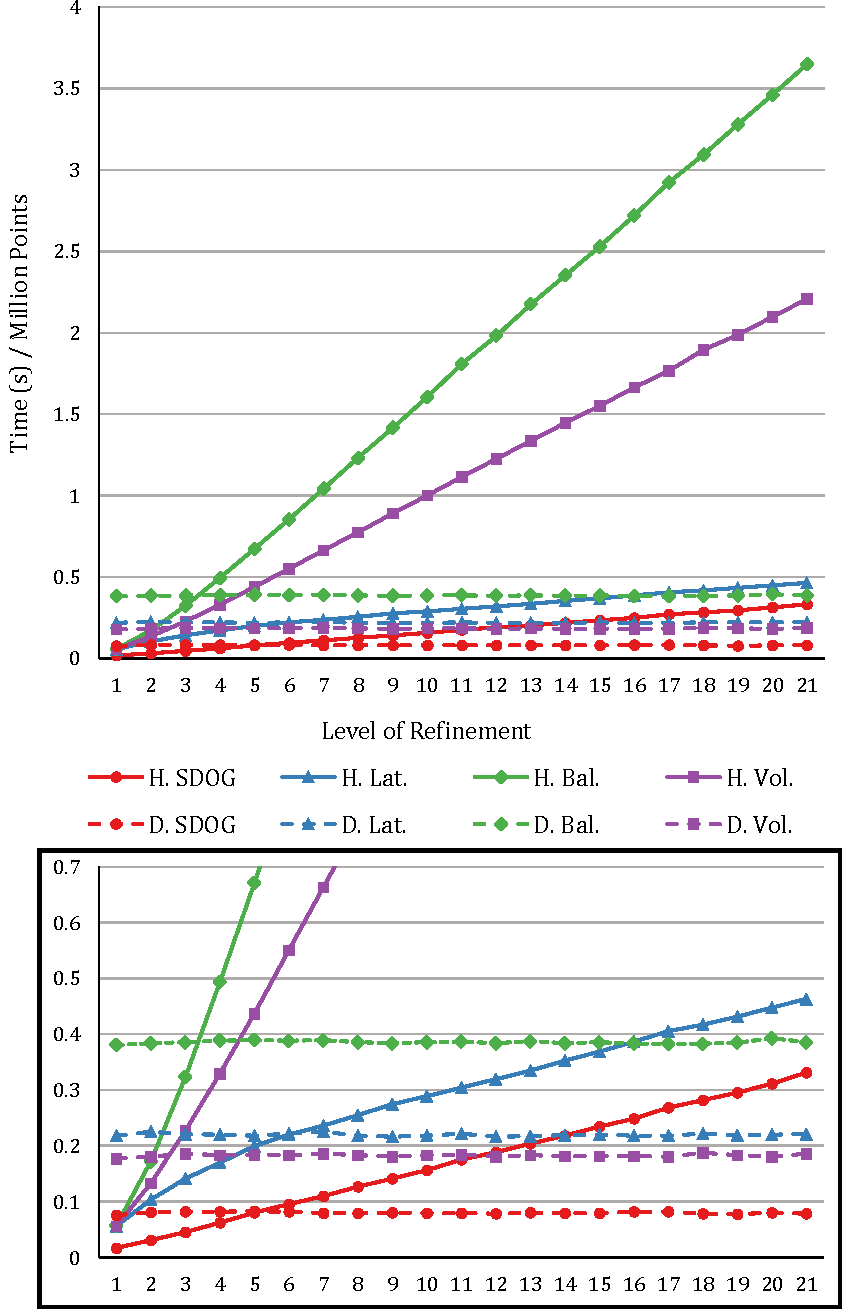
\includegraphics[width=0.8\textwidth]{point-to-index.pdf}
	\caption[Runtime comparison of SDOG point encoding algorithms]{
		A caption will go here.
		The caption may be long.
		This is text that is filling space so that this placeholder caption is longer than if the text was not here.
		Caption caption caption.
		Now the text will repeat...
		A caption will go here.
		The caption may be long.
	}
	\label{fig:point-to-index}
\end{figure}


\begin{figure}[htp!]
	\centering
	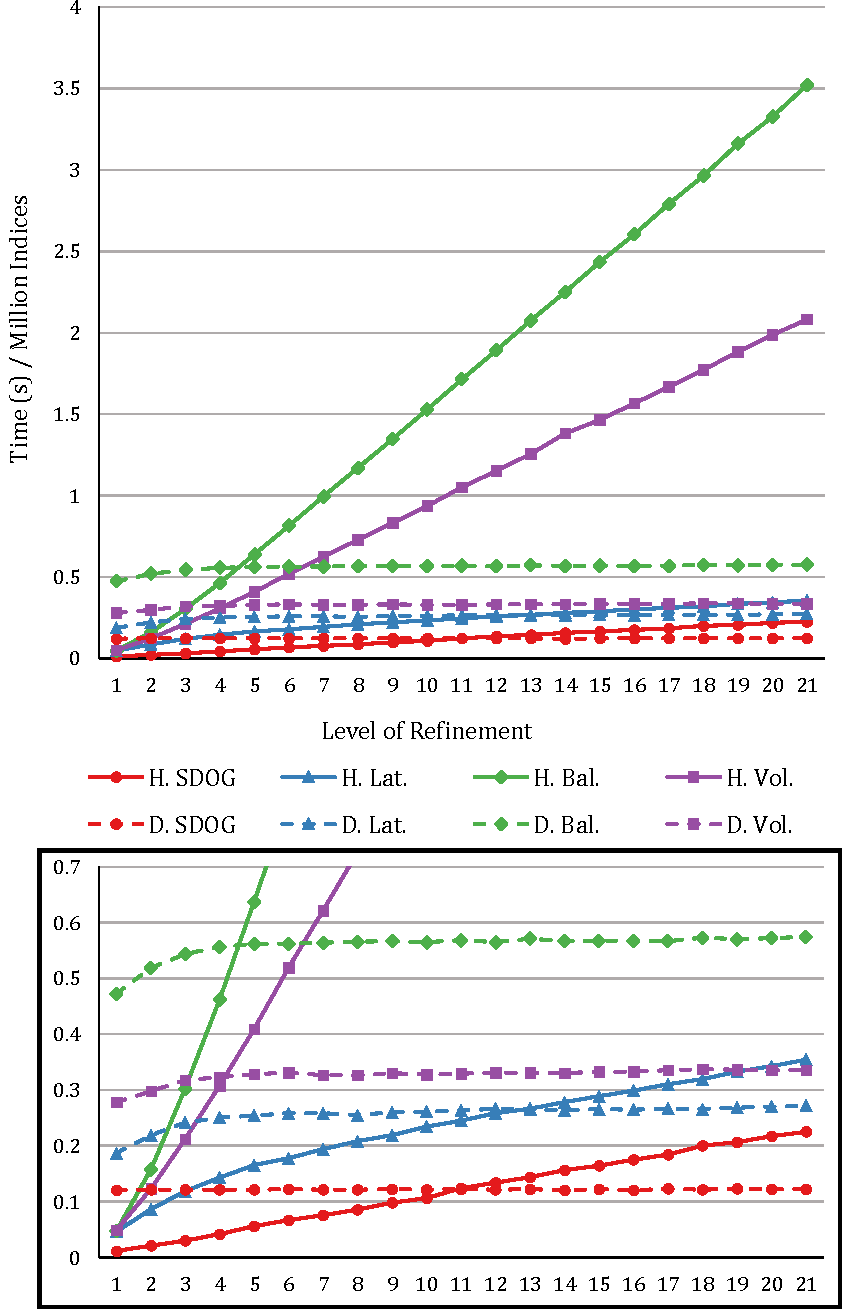
\includegraphics[width=0.8\textwidth]{index-to-range.pdf}
	\caption[Runtime comparison of SDOG decoding algorithms]{
		A caption will go here.
		The caption may be long.
		This is text that is filling space so that this placeholder caption is longer than if the text was not here.
		Caption caption caption.
		Now the text will repeat...
		A caption will go here.
		The caption may be long.
	}
	\label{fig:index-to-range}
\end{figure}


Discussion of the results will go here.


\subsection{Other Indexing Operations}
Parent trivial.
Children trivial if have cell type. SG if $r_i = 2^k - 1$. LG if $\varphi_i = 2^{k - k_\varphi} - 1$.
Neighbours are tricky...


\section{Extension Method}


\subsection{Encoding}


\subsection{Decoding}


\subsection{Other Indexing Operations}
An important component of a conventional DGGS is the indexing scheme for cells.
Indices in a DGGS are used to not only identify and linearize cells but also as a means of navigating the grid for various spatial queries~\cite{alderson2020digital}.
To this end, it is important to be able to perform certain operations on said indices efficiently.
The most fundamental of these operations are parent queries, which return the parent (or with non-congruent refinement, \textit{parents}) of a given cell; child queries, which return the children of the cell; and neighbour queries, which return cells that share an edge (or in 3D a face) with the cell.
These operations serve as the building blocks for more complex geospatial queries done with the grid system, such as region growing, data convolution and correlation, feature rasterization, and buffering.
Because of this, creating suitable indexing for a 3D DGGS is an essential task.


With our method---similar to encoding and decoding---we define these operations in terms of surface and radial components.
This split not only simplifies the problem of indexing but also ensures the 3D indexing is consistent with that of the input DGGS.
Referring back to Figures~\ref{fig:indexing} and \ref{fig:3d-coding}, we let $i_s$ be the surface index of a cell and $i_\ell$ be the layer index.
For each of these components, we assume there is a corresponding parent, child, and neighbour operation.
For the surface index, this comes directly from the input DGGS indexing, whereas for the layer index, these would need to be defined.
Using the component operations, we define the corresponding 3D operations as follows.


\subsubsection{Layer Algorithms}
Parent, child, and neighbours for layers.


\subsubsection{Combined Algorithms}
Combine operations of layers and input to make full 3D operations.


\paragraph{Parents}
The parent(s) of a cell depend on if the layer of the cell and its parent layer have the same, or different, values of $k_s$.
Let $i_\ell' = \operatorname{parent}(i_\ell)$; if the value of $k_s$ is the same, then the single parent is simply $(i_s, i_\ell')$.
In most cases, the value of $k_s$ for $i_\ell'$ is some number $m$ (often one, but not always) less than that of $i_\ell$.
In this case, the parent(s) are given by $\operatorname{parents}^m(i_s) \times i_\ell$.


\paragraph{Children} The children of a cell depend on if the cell belongs to a central or normal layer.
For normal layers, the set of children is simply $\operatorname{children}(i_s) \times \operatorname{children}(i_\ell)$.
For central layers, the child who belongs to the new central layer must be distinguished from the other child layer(s).
Call the index of the new central layer $c_\ell$; then, this child is given by $(i_s, c_\ell)$.
Let $ N_\ell$ give the set of the other children layer indices (normal layers).
These layers have the surface refinement applied $w$ times, so the resulting children are $\operatorname{children}^w(i_s) \times N_\ell$


\paragraph{Neighbours} We split neighbours into three categories: neighbours in the same layers as the cell, neighbours in the layer above the cell, and neighbours in the layer below the cell.
If a cell belongs to the outermost or innermost (central) layer, then it will not have neighbours in the layer above or below, respectively.
Neighbours in the same layer are simply $\operatorname{neighbours}(i_s) \times i_\ell$.
Let $i_\ell^+$ be the layer above $i_\ell$ and $i_\ell^-$ be the layer below.
If $i_\ell^+$ has the same value of $k_s$ as $i_\ell$, then the single neighbour above is $(i_s, i_\ell^+)$.
In the other case, where the value of $k_s$ for $i_\ell^+$ is some number $m$ greater than that of $i_\ell$, the neighbours are given by $\operatorname{children}^m(i_s) \times i_\ell^+$.
Likewise, if $i_\ell^-$ has the same value of $k_s$ as $i_\ell$, there is one neighbour below given by $(i_s, i_\ell^-)$.
In the case that the value of $k_s$ for $i_\ell^-$ is some number $m$ less than that of $i_\ell$, the neighbours are given by $\operatorname{parents}^m(i_s) \times i_\ell^-$

\section{Summary}
A summary of everything will go here.